\section*{Review Questions}

\subsection*{Part A}

\begin{enumerate}
\item Use the Venn diagram below to answer the questions.

\begin{center}
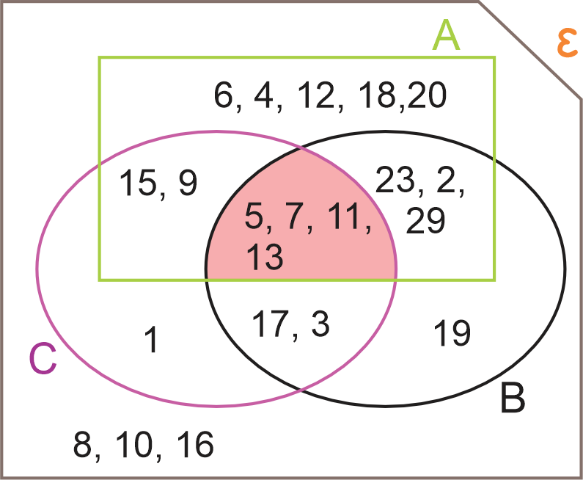
\includegraphics[width=0.55\textwidth]{figures/exercise-q1.png}
\end{center}

\begin{enumerate}
  \item[a.] List the elements in $A$, $B$ and $C$.
  \item[b.] List the elements in $A'$, $B'$ and $C'$.
  \item[c.] Find (i) $(A\cup B\cup C)'$ \quad (ii) $A'\cap B'\cap C'$ \quad (iii) $(A\cap B\cap C)'$ \quad (iv) $A'\cup B'\cup C'$.
  \item[d.] Compare your result in (c)(i) to (c)(ii). What conclusion can you draw?
  \item[e.] Compare your result in (c)(iii) to (c)(iv). What conclusion can you draw?
  \item[f.] Describe set $B$.
  \item[g.] Describe set $C$.
\end{enumerate}

\item Study the diagram carefully and use it to answer the questions.

\begin{center}
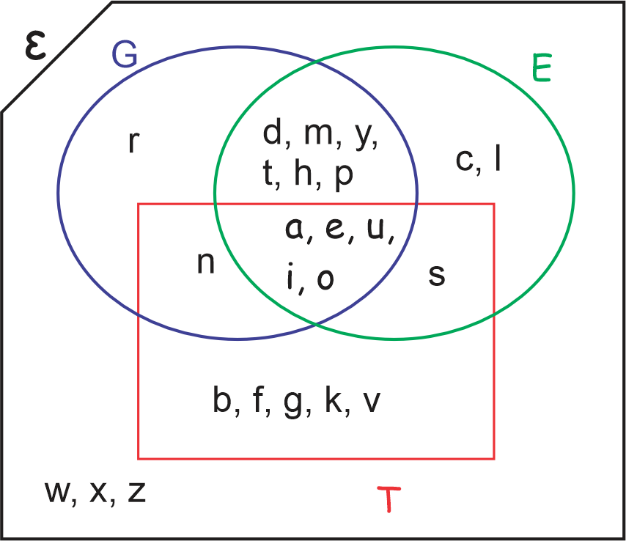
\includegraphics[width=0.55\textwidth]{figures/exercise-q2.png}
\end{center}

\begin{enumerate}
  \item[a.] List the elements in $G$, $E$, $T$ and $\varepsilon$.
  \item[b.] Show that $G' \cap E' = (G\cup E)'$.
  \item[c.] Show that $(G\cap E\cap T)' = G'\cup E'\cup T'$.
  \item[d.] Show that $(G\cup E\cup T)' = G'\cap E'\cap T'$.
\end{enumerate}

\end{enumerate}

\noindent For questions 3--7, sets $X$, $Y$ and $Z$ are subsets of the universal set $\mu$.
Use the information to choose the correct answer to the questions.

\begin{enumerate}[resume]
\item Find $X \cup X'$. \\
\textbf{A.} $\varnothing$ \quad \textbf{B.} $\mu$ \quad \textbf{C.} $X$ \quad \textbf{D.} $Y$

\item Find $Z \cap Z'$. \\
\textbf{A.} $\varnothing$ \quad \textbf{B.} $\mu$ \quad \textbf{C.} $Z$ \quad \textbf{D.} $X$

\item Find $(Y')'$. \\
\textbf{A.} $\varnothing$ \quad \textbf{B.} $\mu$ \quad \textbf{C.} $X$ \quad \textbf{D.} $Y$

\item Find $(X\cup X')'$. \\
\textbf{A.} $\varnothing$ \quad \textbf{B.} $\mu$ \quad \textbf{C.} $X$ \quad \textbf{D.} $X'\cup X$

\item Find $(Z\cap Z')'$. \\
\textbf{A.} $\varnothing$ \quad \textbf{B.} $\mu$ \quad \textbf{C.} $X\cup Y$ \quad \textbf{D.} $Z'\cap Z$

\item Rewrite:
\begin{enumerate}
  \item[a.] $(R\cup S')'$
  \item[b.] $(M'\cap N)'$
  \item[c.] $[(A'\cup B)'\cap C]'$
  \item[d.] $[(P\cap Q')'\cup P]'$
  \item[e.] $[A\cap(A'\cup B)']'$
\end{enumerate}

\item Show that
\begin{enumerate}
  \item[a.] $[(R\cup M)'\cap P]' = R\cup M\cup P'$
  \item[b.] $[(R\cap M)\cup M']' = R'\cap M$
\end{enumerate}

\item On a Venn diagram, shade the region represented by:
\begin{enumerate}
  \item[a.] $(A\cap B)'\cap C$
  \item[b.] $A'\cup(Y\cap Z')$
\end{enumerate}

\item Sets $X = \{\text{prime numbers}\}$, $Y = \{W : 0 < W \le 11\}$ and
$Z = \{1,2,3,4,5,6,7,13,14,15,16,18\}$ are subsets of $A = \{0,1,2,3,4,\ldots,21\}$.
\begin{enumerate}
  \item[a.] List the members of the following sets:
  \begin{enumerate}
    \item[i.] $X$
    \item[ii.] $Y$
    \item[iii.] $X\cap Y\cap Z$
    \item[iv.] $X\cup Y'$
    \item[v.] $(X\cup Y)\cap Z'$
    \item[vi.] $(X'\cap Y)\cup Z$
  \end{enumerate}
  \item[b.] Use a Venn diagram to represent $X$, $Y$, $Z$ and $A$.
\end{enumerate}

\item A survey of 90 teachers reveals the following. 45 teach Management, 57
Accounting and 50 Costing. 25 teach Management and Accounting, 35 teach
Accounting and Costing and 22 teach Management and Costing. 5 teachers
cannot teach any of the three subjects.
\begin{enumerate}
  \item[a.] Represent the information on a Venn diagram.
  \item[b.] Calculate the number of teachers who can teach only one of the three subjects.
\end{enumerate}

\item A survey of 41 employees shows that 25 are skilled in Carpentry, 15 in
Brick laying and 24 in Tiling. 12 are skilled in carpentry and brick laying,
9 in brick laying and tiling, 17 in carpentry and tiling, and 8 are not
skilled in any of the three occupations. Find the number of employees who
are skilled in
\begin{enumerate}
  \item[a.] all three occupations
  \item[b.] exactly two of the occupations
\end{enumerate}

\item A class of 60 students were each required to have textbooks in Accounting,
Management and Costing. However, when the class teacher checked their
books, she found out that: 16 had Accounting and Management books, 14
had Accounting and Costing books, 18 had only two of the three books and
20 had Accounting plus at least one other book. Every student had at
least one of the three books. Find the number of students who had
\begin{enumerate}
  \item[a.] all three books.
  \item[b.] only Costing and Accounting books.
  \item[c.] exactly one of the three books.
  \item[d.] If 16 students had neither Accounting nor Costing books, find the
  probability that a student selected at random from the class had Management books.
\end{enumerate}

\item The analysis of results of a sample of students who sat for the WASSCE
in Biology, Physics and Mathematics revealed that: 80\% passed in Biology,
65\% passed in Mathematics, 70\% passed in Physics, 52\% passed in Biology
and Mathematics, 58\% passed in Biology and Physics, 55\% passed in
Physics and Mathematics, 45\% passed in all three subjects. What
percentage of the students:
\begin{enumerate}
  \item[a.] passed only Mathematics
  \item[b.] passed only Physics
  \item[c.] passed only Biology
  \item[d.] passed Biology and Physics but not Mathematics
  \item[e.] did not pass any of the subjects.
\end{enumerate}

\item A shop owner kept records of purchases made by customers over the
weekend. The shop sells food, clothing and hardware. She found that, out
of the customers who visited her shop, 210 purchased food products, 100
hardware and 147 clothing. 30 purchased food and hardware. 128 purchased
two of the three products. She also found that of those who purchased two
of the three products, 14 did not buy clothing and 20 did not buy food. 13
of the customers who visited the store did not buy any of the products.
\begin{enumerate}
  \item[a.] How many customers visited the store over the weekend?
  \item[b.] How many of the customers who visited the store:
  \begin{enumerate}
    \item[i.] purchased less than two products.
    \item[ii.] purchased all three products.
    \item[iii.] purchased food and other products.
  \end{enumerate}
\end{enumerate}

\item A group of 210 tourists were asked to indicate which of the languages,
German, French and English they can speak. It was found that 55 can
speak German, 76 can speak French and 200 can speak English. 103 can
speak two of the three languages and 6 tourists cannot speak any of the
three languages. Find the number of tourists who can speak:
\begin{enumerate}
  \item[a.] all three languages
  \item[b.] only one of the three languages.
\end{enumerate}

\item 87 schools in Tamale have subscriptions to at least one of the following
newspapers: Graphic, Mirror and Times. 69 subscribe to Graphic, 62 to
Mirror and 55 to Times. 32 have subscriptions to all three newspapers.
Find the number of schools who have subscriptions to:
\begin{enumerate}
  \item[a.] exactly two of the newspapers
  \item[b.] only one of the newspapers.
\end{enumerate}

\item A publishing company surveyed its employees about their proficiency in
three software: Photoshop, CorelDraw and InDesign. The results show that
all the employees were proficient in at least one of the three software and
10 were proficient in all three. The number of employees proficient in
CorelDraw and other software were twice those proficient in only
CorelDraw. Of the employees who were proficient in two of the software,
14 were not proficient in InDesign, 8 were not proficient in CorelDraw and
6 were not proficient in Photoshop. The same number of employees
proficient in only InDesign are proficient in only Photoshop. There were
more employees proficient in only Photoshop and InDesign than employees
proficient in only Photoshop and there were fewer employees proficient in
only InDesign and CorelDraw than employees proficient in only InDesign.
\begin{enumerate}
  \item[a.] Use a Venn diagram to represent the above data.
  \item[b.] How many employees were involved in the survey?
  \item[c.] How many employees were proficient in only one of the software?
\end{enumerate}

\end{enumerate}

\subsection*{Part B}

\begin{enumerate}
\item Write down the first five terms of the binomial expansion of:
\begin{enumerate}
  \item[a.] $(1+4x)^{12}$
  \item[b.] $(1-3x)^9$
  \item[c.] $(3+2x)^7$
  \item[d.] $\left(1-\dfrac{x}{2}\right)^8$
  \item[e.] $\left(2-\dfrac{5}{2}x\right)^6$
\end{enumerate}

\item Write down the term indicated in the binomial expansion of the following
functions:
\begin{enumerate}
  \item[a.] $(1+3x)^6$: 3rd term
  \item[b.] $\left(1+\dfrac{x}{3}\right)^{20}$: 7th term
  \item[c.] $(a+4b)^{12}$: term containing $a^4$
\end{enumerate}

\item Expand the following binomial expansions up to and including the terms
in $x^2$:
\begin{enumerate}
  \item[a.] $(1-2x)(1+x)^8$
  \item[b.] $(2+3x)(1+3x)^{10}$
  \item[c.] $(5+2x)\left(1-\dfrac{2}{3}x\right)^{12}$
  \item[d.] $(1+4x)(1-3x)^{20}$
\end{enumerate}

\item Expand $(1-2x)^7$ and hence find the value of $(0.98)^7$ correct to 4 decimal
places.

\item Find the first four terms of the following using the binomial theorem.
\begin{enumerate}
  \item[a.] $\left(1-\dfrac{1}{2}x\right)^{1/2}$
  \item[b.] $(1-2x)^{-3}$
  \item[c.] $(3-x)^{-2}$
\end{enumerate}

\item Use appropriate binomial expansions to find the approximate values of:
\begin{enumerate}
  \item[a.] $\sqrt[3]{8.7}$ correct to 5 significant figures.
  \item[b.] $(81.162)^{1/4}$ to 4 decimal places.
  \item[c.] $\sqrt{4.02}$ to 3 decimal places.
  \item[d.] $\dfrac{1}{\sqrt{10}}$ to 4 decimal places.
  \item[e.] $\sqrt{101}$ to 4 decimal places.
  \item[f.] $(0.995)^5$ to 4 decimal places.
\end{enumerate}

\item Show that in ascending powers of $x$, $\left(\dfrac{1-x}{1+x}\right)^{1/3}$ is
$1 - \dfrac{2}{3}x + \dfrac{2}{9}x^2 - \dfrac{4}{21}x^3 - \cdots$.

\item Expand the following as far as the $x^3$ term:
\begin{enumerate}
  \item[a.] $(1+x+2x^2)^3$
  \item[b.] $(1+3x+x^2)^4$
\end{enumerate}

\item
\begin{enumerate}
  \item[a.] Find the first 3 terms in ascending powers of $x$ of the binomial
  expansion $(1+py)^9$, where $p$ is a non-zero constant.
  \item[b.] If the first 3 terms are $1$, $36x$ and $qx^2$ where $q$ is a constant, find
  the value of $p$ and $q$.
\end{enumerate}

\item
\begin{enumerate}
  \item[a.] Find the first 3 terms in ascending powers of $x$ of the binomial
  expansion $(2+kx)^7$, where $k$ is a constant.
  \item[b.] Given that the coefficient of $x^2$ is 6 times the coefficient of $x$, find
  the value of $k$.
\end{enumerate}

\end{enumerate}
